\documentclass[12pt]{article}

%packages
\usepackage[usenames,dvipsnames,table,xcdraw]{xcolor}
\usepackage{multirow}
\usepackage{fullpage}
\usepackage{tikz}
\usepackage{amsmath}
\usepackage{graphics}
\usepackage{makeidx}

\makeindex

%commands
\newcommand{\notes}[1]{{\color{Tan} #1}}
\newcommand{\emdex}[1]{\emph{#1}\index{#1}}
\newcommand{\peupfudge}{Peupfudge}

\title{\peupfudge}
\author{Ebrahim \\ Yusuf \\ Yussra}
\date{\today}

\parindent0ex
\parskip5mm


\begin{document}
%\maketitle
\textbf{\peupfudge}
\hfill
\textbf{\today}\\
\textit{Derived from core Fudge rules by Ebrahim, Yusuf, and Yussra.}

\setcounter{tocdepth}{2}
\tableofcontents

\section{Introduction}
\notes{what peupfudge is all about.
it gives you the classes and not the objects.
what a gm is.
pc vs npc.
xp.
how we suggest you read this manual.}

\subsection{Numbers and Adjectives} \label{sec:quant}

%we quantify challange and capability
Players will face challenges, and they will have to rely on the capabilities of their
characters to confront them.
At its core, \peupfudge{} is nothing more than a mechanism 
that crudely quantifies these challenges and capabilities in order to
compare them and weave an interesting narrative.
Let us set up the numerical scale to be used for this quantification:
\begin{center}
{\setlength{\extrarowheight}{1pt}
\begin{tabular}{l|l}
level & adjective \\
\cline{1-2}
-4 & abysmal \\
-3 & terrible \\
-2 & poor \\
-1 & mediocre \\
0  & fair \\
1  & good \\
2  & great \\
3  & superb \\
4  & legendary \\[8pt]
%\multicolumn{2}{c}{(more levels may be introduced if needed)}
\end{tabular}}
\end{center}
We call these numbers \emph{levels}; they appear as ability levels in section \ref{sec:tree}
and as difficulty levels in section \ref{sec:actions}.
The adjectives provide some guidelines for interpreting levels.
This interpretation is sharpened by viewing the scale as
logarithmic with a base of \input{base.tex}\unskip.
This means that a good climber is \input{base.tex} times as skilled as a fair climber,
who is in turn \input{base.tex} times as skilled as a mediocre climber, and so on.
A cliff of good difficulty level can be thought of as one that would challenge a good climber,
in that a good climber would be expected to successfully climb it $38\%$ of the time.

What does it even \emph{mean} to say things like $A$ is ``twice as good of a climber'' as $B$?
We take it to mean that $A$ has about twice the climbing experience that $B$ has.
Making sense of this in turn requires that we agree on some sort of untrained baseline for climbing.
This baseline should be based on the adjective that makes sense, and the GM chooses it
explicitly while building the ability tree (coming up in section \ref{sec:tree}).

Some care is needed in order to interpret levels consistently.
Suppose that $A$ has great strength and $B$ has merely good strength.
This apparently means that ``$A$ is \input{base.tex} times as strong as $B$.''
But this does \emph{not} imply that $A$ can lift \input{base.tex} times as much weight as $B$.
What it does imply is that the factor by which $A$ can lift more weight than $B$ is
\emph{as though} $A$ had \input{base.tex} times as much strength training \emph{experience} as $B$.
If the skill in question were running, then $A$ would not be \input{base.tex}
times faster than $B$, but rather have \input{base.tex}
times as much running experience.

\paragraph{Orders}
So ability levels correspond to the experience required to attain a certain degree of competence... but \emph{whose} experience?
If all characters in a campaign are humans, then the focus is on human experience.
But how could one measure, say, a giant's strength in terms of the amount of experience a human needs to attain such strength?
It may well be that \emph{no} amount of strength training could bring an ordinary human to such strength.
Giants are simply on a different scale of numbers when it comes to the level of their strength ability;
we will say that their strength is of a different \emdex{order}.
\begin{center} 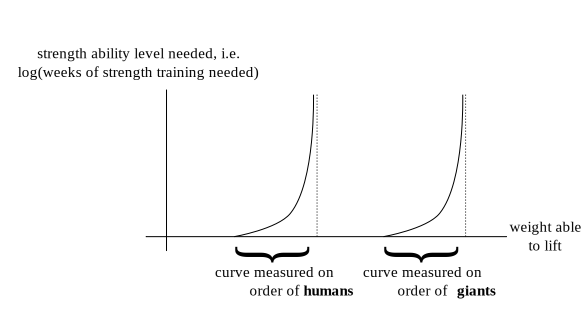
\includegraphics{svg/orders.eps} \end{center}
For each order that is needed in a campaign, the GM should assign a label that looks like a unit of measurement.
For example a giant of great strength (for a giant) would be said to have strength $2$G,
where the label ``G'' indicates that the level $2$ is meant to be interpreted on the order of giants.
Unlabeled ``unitless'' levels should be interpreted on the order of humans, or whatever is the
\emdex{standard being}, the most typical type of creature that can serve as a player character within a campaign.


%3 things help interpret: adj, b times xp, 38%
To summarize, there are four elements that can provide information on a level:
\vspace{-1em}\begin{enumerate}
\item The adjective that goes with the level.
\item The order label on the level.
\item The interpretation of relative ability levels
(each additional ability level corresponds to
\input{base.tex} times as much experience's worth of the ability).
\item The probability governing difficulty levels
(a challenge of difficulty level $D$ is one that can be overcome $38\%$ of the time for
someone with an ability level of $D$).
\end{enumerate}
%gm needs to know how to judge the difficulty of a task,
%and also gm and players need to know how to interpret for narrative sake
The GM ought to understand levels in order to judge the difficulties of various tasks
and add appropriate modifiers to various rolls.
The players should also understand levels to some extent,
so that their perception of the shared narrative coalesces and lines up with the mechanics
of \peupfudge{}.

%dF
We will refer to dice rolls using the ``d$n$'' notation,
which stands for an $n$-sided die.
The main die type used here is the \emdex{fudge die},
which can yield $-1$, $0$, or $+1$ with equal chances.
We denote a fudge die roll by ``dF.''
The result of a roll of $N$ fudge dice ($N$dF) is the sum of the results of the individual die rolls.


\section{Characters}
A \emph{character}
\index{character} is an agent in the world.
Individual characters are represented by their traits,
which describe a character's background, abilities, and their dynamic current state.

\index{traits}
\textbf{Traits}\vspace{-1em}
\begin{itemize}
\item \emph{Characteristics}
describe identity and background
(e.g., name, race, species, height, gender).
\item \emph{Abilities}
represent improvable traits that play a role in action resolution
(e.g. strength, climbing, legal knowledge).
They have an integer ability level.
\emph{Powers} are abilities that can be turned off completely.
Abilities are organized in a tree and separated into \emph{skills} and \emph{attributes} (see section \ref{sec:tree}).
\item \emph{Properties} are binary traits-- a character either has or does not have a given property
(e.g. deaf, blessed).
\item \emph{Bars} are other statuses that need constant tracking (e.g. mana, hunger, reputation).
\item \emph{Health} is the set of conditions that describe the state of a character's well-being.
\item \emph{Inventory} is the collection of items on a character's person.
\end{itemize}


In creating a game world, a GM needs to specify the traits relevant to the campaign.
A GM must essentially decide how a character sheet looks.
In particular, this will involve inventing some of the traits, which might be based on the specific setting of the game.

\subsection{The Ability Tree}\label{sec:tree}			

The purpose of an ability level is to have something to roll against while resolving actions.
(Action resolution will be covered in section \ref{sec:actions}.)

Ability levels are to be interpreted based on section \ref{sec:quant}.
%abilities starting at poor
Most abilities have an initial (untrained) level of -2.
The GM may choose some different initial ability levels based on the difficulty of a skill.
An ability that is hard to pick up might have an initial level of -3, while an easy ability could start at -1.
\index{ability!starting level}

%define structure of tree, as well as terms 'skill' and 'attribute'
Abilities are arranged in a tree structure in which broad abilities govern more specific ones.
\index{ability!ability tree}
An ability that governs others is an \emph{attribute} (a non-terminal node), while an ability that does not govern any others is a \emph{skill} (a terminal node).
\index{skill}\index{attribute}
Each arrow of the tree (each governing of one ability by another) has an associated \emph{weight}.
\index{weight}
\index{ability!weight}
Weight represents the impact an ability has on its group, i.e. the degree to which its improvement
in turn improves its governing attribute.
Below is an example of an initial ability tree, with an ability level written next to each ability.
Attributes are shown in blue, skills are shown in red, and weights are labeled on the arrows.

\begin{center}
% THIS FILE WAS AUTOMATICALLY GENERATED BY gen_trees.py

\tikzset{
  treenode/.style = {shape=rectangle, rounded corners, top color=white, draw},
  attribute/.style     = {treenode, font=\ttfamily\normalsize, bottom color=blue!30},
  skill/.style         = {treenode, font=\ttfamily\normalsize, bottom color=red!20, right},
  weight/.style = {pos=0.5, shape=circle, scale=1, minimum height=1, inner sep=1pt, fill=white, font=\scriptsize, draw}
}
\begin{tikzpicture}
\draw
  (0,-3.08125) node [attribute] (level) {level -2} 
  (3,-1.0625) node [attribute] (mind) {mind -2} 
  (9.5,0) node [skill] (engineering) {engineering -4} 
  (9.5,-0.85) node [skill] (literacy) {literacy -2} 
  (6.5,-2.125) node [attribute] (medicine) {medicine -3} 
  (9.5,-1.7) node [skill] (wound care) {wound care -3} 
  (9.5,-2.55) node [skill] (first aid) {first aid -2} 
  (3,-5.1) node [attribute] (body) {body -2} 
  (6.5,-3.825) node [attribute] (muscle) {muscle -2} 
  (9.5,-3.4) node [skill] (hand-to-hand) {hand-to-hand -2} 
  (9.5,-4.25) node [skill] (hauling) {hauling -2} 
  (9.5,-5.1) node [skill] (climbing) {climbing -3} 
  (6.5,-6.375) node [attribute] (athletics) {athletics -2} 
  (9.5,-5.95) node [skill] (swimming) {swimming -3} 
  (9.5,-6.8) node [skill] (running) {running -1} 
;
\draw[-{latex}] (level) -- (mind.west)  node[weight]{1};
\draw[-{latex}] (level) -- (body.west)  node[weight]{1};
\draw[-{latex}] (mind) -- (engineering.west)  node[weight]{1};
\draw[-{latex}] (mind) -- (literacy.west)  node[weight]{2};
\draw[-{latex}] (mind) -- (medicine.west)  node[weight]{1};
\draw[-{latex}] (medicine) -- (wound care.west)  node[weight]{1};
\draw[-{latex}] (medicine) -- (first aid.west)  node[weight]{1};
\draw[-{latex}] (body) -- (muscle.west)  node[weight]{2};
\draw[-{latex}] (body) -- (climbing.west)  node[weight]{1};
\draw[-{latex}] (body) -- (athletics.west)  node[weight]{2};
\draw[-{latex}] (muscle) -- (hand-to-hand.west)  node[weight]{1};
\draw[-{latex}] (muscle) -- (hauling.west)  node[weight]{1};
\draw[-{latex}] (athletics) -- (swimming.west)  node[weight]{1};
\draw[-{latex}] (athletics) -- (running.west)  node[weight]{1};
\end{tikzpicture}
\end{center}

\paragraph{The Idea} Let us summarize the mechanics to be explained.
Players are granted experience points (xp) throughout the game.
They may use xp to raise skills that they have recently used (i.e. rolled against).
\index{xp}
Only skills, and not attributes, may be raised directly with xp.
The mechanics of training abilities are such that competence in skills related to a given skill makes it easier to train that skill.
Consequently, players are encouraged
to make characters that make sense and have some degree of specialization.


%parent ability makes it easier to train children. need to consider full ancestral line. explain 'xp' or refer to sec:dev. give table and equation. note that poor parents are like no parents.
\subsubsection{Training Skills}\label{sec:skill}
\index{train}\index{xp}
The xp cost of raising a particular skill level depends on
the skill's current level and the levels of all its ancestor attributes in the ability tree.
A high-level skill is harder to raise.
A skill with high-level governing attributes is easier to raise.
%(I deleted "because it implies related knowledge" b/c we already said that in the conceptual summary -e)
Use the following table to determine the xp cost for a skill level increase:

\begin{center}
\resizebox{\columnwidth}{!}{
\input{xptable.tex}
}
\end{center}
%I don't like using the standard roman font in the table. should find a better font to display those numbers


The \emph{attribute bonus} is a weighted average over all ancestor attributes of the skill being trained:
\index{attribute bonus}
\begin{align*}
\textrm{[attribute bonus]}
=\big(\ &\textrm{[level of governing attribute]}\\
&+\ \frac{1}{2}\textrm{[level of its governing attribute]}\\
&+\ \frac{1}{4}\textrm{[level of its governing attribute]}\\
&+\ \cdots \big)
\ /\ \big(1+\frac{1}{2}+\frac{1}{4}+\cdots\big)
\end{align*}
Thus, the closer an attribute is to a skill in the ability tree, the larger its hand in governing the skill. 





%raising child ability level has chance of raising parent. this applies to attributes as well. give formula and way to implement.
\subsubsection{Training Attributes}\label{sec:att}
Unlike skills, attributes cannot be trained directly by using xp.
\index{train}
Whenever an ability level is increased, there is a chance that its governing ability will also increase.
This mechanic applies to \emph{all} abilities, so that the effect of training skills via xp
propagates up the ability tree in a probabilistic fashion.
Here's how it works:
Let $A$ be an attribute that governs abilities $B_1,\ldots,B_n$, with respective weights $w_1,\ldots, w_n$.
Whenever $B_i$ increases in level, the chance that $A$ increases in level is given by
$$\frac{w_i}{w_1+\cdots+w_n}\ .$$
It is sensible to round this quantity to the nearest $(\frac{1}{n})^\text{th}$ and roll a d$n$ to determine
whether or not $A$ increases in level.
\index{ability!weight!dice roll}
In fact, this quantity only needs to be computed once for each arrow of the ability tree,
and the weights can then be dispensed with.
After choosing initial weights and computing these probabilities,
one might as well label the arrows by the dice roll one needs to surpass to raise a governing attribute.
We recommend that the GM present the game's ability tree to players in this format.
To demonstrate, here is our example tree from earlier, with d20 difficulties on the arrows:
\begin{center}
% THIS FILE WAS AUTOMATICALLY GENERATED BY gen_trees.py

\tikzset{
  treenode/.style = {shape=rectangle, rounded corners, top color=white, draw},
  attribute/.style     = {treenode, font=\ttfamily\normalsize, bottom color=blue!30},
  skill/.style         = {treenode, font=\ttfamily\normalsize, bottom color=red!20, right},
  weight/.style = {pos=0.5, shape=rectangle, scale=1, minimum height=1, inner sep=2pt, fill=white, font=\scriptsize, draw}
}
\begin{tikzpicture}
\draw
  (0,-3.08125) node [attribute] (level) {level -2} 
  (3,-1.0625) node [attribute] (mind) {mind -2} 
  (9.5,0) node [skill] (engineering) {engineering -4} 
  (9.5,-0.85) node [skill] (literacy) {literacy -2} 
  (6.5,-2.125) node [attribute] (medicine) {medicine -3} 
  (9.5,-1.7) node [skill] (wound care) {wound care -3} 
  (9.5,-2.55) node [skill] (first aid) {first aid -2} 
  (3,-5.1) node [attribute] (body) {body -2} 
  (6.5,-3.825) node [attribute] (muscle) {muscle -2} 
  (9.5,-3.4) node [skill] (hand-to-hand) {hand-to-hand -2} 
  (9.5,-4.25) node [skill] (hauling) {hauling -2} 
  (9.5,-5.1) node [skill] (climbing) {climbing -3} 
  (6.5,-6.375) node [attribute] (athletics) {athletics -2} 
  (9.5,-5.95) node [skill] (swimming) {swimming -3} 
  (9.5,-6.8) node [skill] (running) {running -1} 
;
\draw[-{latex}] (level) -- (mind.west)  node[weight]{10};
\draw[-{latex}] (level) -- (body.west)  node[weight]{10};
\draw[-{latex}] (mind) -- (engineering.west)  node[weight]{15};
\draw[-{latex}] (mind) -- (literacy.west)  node[weight]{10};
\draw[-{latex}] (mind) -- (medicine.west)  node[weight]{15};
\draw[-{latex}] (medicine) -- (wound care.west)  node[weight]{10};
\draw[-{latex}] (medicine) -- (first aid.west)  node[weight]{10};
\draw[-{latex}] (body) -- (muscle.west)  node[weight]{12};
\draw[-{latex}] (body) -- (climbing.west)  node[weight]{16};
\draw[-{latex}] (body) -- (athletics.west)  node[weight]{12};
\draw[-{latex}] (muscle) -- (hand-to-hand.west)  node[weight]{10};
\draw[-{latex}] (muscle) -- (hauling.west)  node[weight]{10};
\draw[-{latex}] (athletics) -- (swimming.west)  node[weight]{10};
\draw[-{latex}] (athletics) -- (running.west)  node[weight]{10};
\end{tikzpicture}
\end{center}
When a player trains their \emph{climbing} skill by spending the needed xp,
they also roll a d20 to see if their \emph{body} attribute increases.
If they roll more than 16, it does increase.
In this case they would roll again for a chance to increase their \emph{level} attribute,
with success if the roll surpasses 10.


Order\index{order} labels are never added or removed through the training of skills or attributes,
and they have no effect on determining the attribute bonus or reading the xp cost table.





\subsubsection{Tree Design}
The mechanics for training skills and attributes are meant to resemble real training and experience.
\index{train}
Training a specific skill is easier to do given more general related experience,
and more so for the experience that pertains most directly to the skill,
hence the attribute bonus of section \ref{sec:skill}.
At the same time, the general experience typically comes from training in a wide variety of related specific skills,
hence section \ref{sec:att}.

%good tree design is important. if it seems limiting that only skills can be trained directly, then the tree may not be designed well.
Designing a good ability tree may require some practice and repeated revisions at first.
If it seems limiting in the context of a given tree that attributes cannot be trained directly,
then consider redesigning the tree.
Perhaps some of those attributes should instead be skills, and new attributes should be
introduced to group them.
One approach to designing a tree from scratch is to begin by listing all the desired skills
and grouping them into related clumps.
Suitable attributes could take form in the clumps.

An ability tree need not have a single root ability; it could instead
consist of multiple disconnected ability trees.
A reasonable root ability, if one is desired, would be akin to the notion of a ``character level'' common to role playing games.
While it wouldn't mean quite the same thing in the context of an ability tree, \emph{level} is still a compelling name for
what could be thought of as ``general competence'' or ``the ability to learn.''

\paragraph{Powers}
Some abilities can be labeled as \emph{powers}, which just means that they can be disabled completely.
\index{power}
A power that is disabled for a character cannot be trained or rolled against,
but it plays the same role as an ordinary ability for all other purposes (e.g. calculating
the probabilities in section \ref{sec:att}).
All abilities governed by a power are automatically powers, and they are
automatically disabled when the power is disabled.
The GM should decide what sorts of circumstances cause various powers to become enabled.

The option of powers is available because it sometimes makes sense for certain abilities to be altogether unavailable to certain characters.
One could implement such abilities as \emph{properties} instead (explained in section \ref{sec:dev}),
but it may be desirable to incorporate them into the ability tree so that they can be trained and tracked with other abilties.
A typical example would be magic as an innate ability.
\index{magic}
Non-casters should have it disabled in their tree, but one could envision an entire subtree consisting of schools of magic for casters.

\paragraph{NPCs}
Tracking the abilities of every NPC using a full ability tree can become a hassle.
Fortunately, there is an easy way to lessen this work: simply \emph{trim} their ability tree!
That is, shave off some abilities from the skill end of their tree so that some attributes become skills.



\paragraph{Orders}
The GM should ponder over what orders\index{order} of levels might be needed for their campaign.
What are the most standard beings in the world to serve as player characters?
Unlabelled ``unitless'' ability levels are interpreted in terms of these beings,
as described in section \ref{sec:quant}.
Consider each ability in the context of the beings of the world.
Do some of these abilities need special order labels for some of the beings?
The typical situation would be one in which there is an ability $A$ and
two types of beings $B_1$ and $B_2$ such that
levels of $A$ on the order of $B_1$ are never sufficient
to describe the ability $A$ for beings of type $B_2$.


\subsubsection{Belated Tree Augmentation}\label{sec:bta}

In case you find yourself wishing, long after starting a game,
that you had included a certain skill in the ability tree,
we propose some rules for introducing it.
Add the skill in the desired position to every player's tree.
Set the skill's level to 2 below the level of its governing attribute for each player.
Include the desired weight, and recalculate the dice roll difficulties for all skills governed by the governing attribute.


\subsection{Character Development}\label{sec:dev}

The GM should provide players with the structure of an empty character sheet,
complete with all the needed traits to be initialized by players.
While abilities have well-defined mechanics, some other traits
need to be specified and elaborated by the GM.

First we take a moment to explain how xp works throughout gameplay,
then we lay out the different aspects of character creation.

\subsubsection{Using Experience Points}
Experience points (xp) quantify the process of training abilities.\index{xp}
The GM doles out xp to the players after their characters accomplish some chunk of the narrative.
The idea is that more xp should be awarded for greater success and for the accomplishment of more difficult tasks,
but this is ultimately up to the GM.
%xp can only be used to raise skills, not attributes. and only ones that were used (rolled against) lately. (players ask gm).
The purpose of xp is to spend it to increase the levels of skills according to the xp cost table in section \ref{sec:tree}.
Note that attribute levels cannot be raised directly, but instead have a chance of increasing every time a governed skill is trained.

The skills that can be trained should be limited to ones that are relevant to the accomplishments that resulted in the xp reward in the first place.
\index{train}
A GM may enforce this by listing 
(perhaps separately for each player)
which skills have been opened
to xp allocation after a given xp reward,
or by asking players to clear each skill with them.
Players cannot save xp to use on arbitrary skills; they must \emph{allocate} their xp towards skills when they receive it.
It is fine to allocate to a skill an amount of xp less than what is needed to increase its level.
Players are responsible for keeping track of how much xp they have invested in partially purchased skill level increases.

\subsubsection{Character Creation}\label{sec:creation}
Players start with some xp to build up their ability tree. \index{xp}
A reasonable starting quantity is \input{xp_start_multiplier.tex}xp times the number of skills in the tree,
but a GM may have reasons for using more or less, or even for varying the amount for certain characters.
The ability tree a character starts with represents skills
gained during a character's life up to the beginning of the narrative,
so these sorts of GM decisions can be based on other information about the character.
The starting xp is spent during character creation, and it works just like the ordinary character development that follows an xp award.
Since much depends on rolling at this stage, we recommend that it be done ``live;'' i.e. in the presence of other players.
As an alternative to this form of character creation, a GM may provide prepared \emph{classes} for players to pick from.
A \emph{class} is nothing but a pre-made ability tree.
This alternative eliminates rolling completely; a middle ground option would be to provide a choice
of partially developed classes and also give a bit of xp for customization.

Characteristics should also be pinned down during character creation.\index{characteristic}
Since they play a mostly narrative role, there are no detailed mechanics to govern their structure.
The GM simply chooses which characteristics are relevant to the game world, and they are included on character sheets.
Players are encouraged to write descriptions that are brief enough to reference and recall while still
providing sufficient narrative substance to make characters feel real.

Some aspects of a character's description ought to be acknowledged more formally.
They might need to interact with other game mechanics
in a specific way (e.g. a character with no arms should have some trouble training their swordsmanship),
or they might just need to be put in the spotlight due to their effect on many situations
(e.g. a deaf character should have a reduced chance of noticing the ambush they are about to walk into).
This is addressed by one more type of character trait: \emph{properties}.\index{property}
A property should be a label that can be true of a character or not,
and it should have a description if it needs one.
A character's properties should be listed on their character sheet.
Players can come up with properties at character creation and get them approved by the GM.
The GM can also provide a list of properties for players to choose from, with some descriptions and constraints.

A second way to incorporate a character description into the more formal traits
is to make exceptions for the starting levels of certain abilities.
For example, a character who is a mermaid should have a very high initial swimming ability.
The ideas of section \ref{sec:quant} can be used to set these starting levels appropriately.

%bars are other info u want to keep track of
The setting or focus of a campaign might call for the constant tracking of specific
character information for all player characters.
\emph{Bars}\index{bar} can be used
for this purpose.
Examples include hunger, thirst, mana, reputation, mood, sleepiness, fatigue, and hygiene.
For each bar included, the GM should specify a few things:
\vspace{-1em}\begin{itemize}
%specify what the bar means
\item Meaning: What values/states can the bar be in, and what do the different states mean?
%specify what causes a bar to change and how it starts out.
\item Behavior: What causes the bar to change state? Also, how does it start out?
%and specify what its effects are
\item Effects: What are the effects of the bar's being in the various states?
\end{itemize}
Bars are useful when the type of information that needs to be tracked
doesn't qualify as any of the traits we've already introduced;
for example it may not fit as an ability level, it may not be binary like a property,
and it may need more careful attention than a characteristic.
If the behavior of a bar is particularly complicated then it may be better implemented
as a \emdex{condition}, coming up next.

\subsection{Health} \label{sec:health}
A character's health is described entirely by their \emdex{conditions}.
Conditions that could afflict a character have a pre-defined progression represented by a flowchart.
For every creature in their world, the GM should consider what health conditions they wish to include.
\emph{States}\index{state} are collections of symptoms, effects on afflicted characters.
They are represented in the flowchart by nodes.
\emph{Transitions}\index{transition} between states are specified by saying the circumstances that trigger them
and the way to determine the resulting state.
They are represented in the flowchart by arrows that branch to nodes for potential resulting states.
Arrows with no source node represent the cause(s) of a condition, the ways for a character to develop the condition.
Here is an example flowchart for the condition of tuberculosis:

\begin{center} 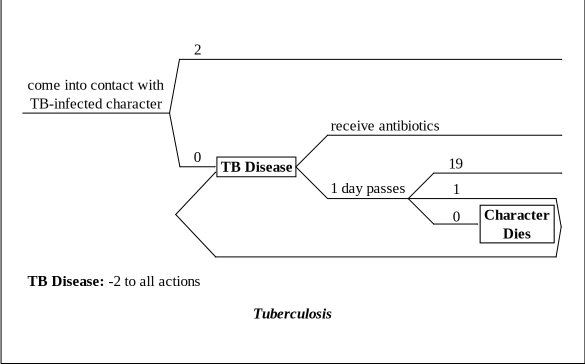
\includegraphics{svg/tb.eps} \end{center}

The numbers in this example are used to represent d$20$ rolls used to determine the outcome of a transition. 
We have used a notation in which the outcome is the one with the highest value surpassed by a d$20$ roll.
Suppose a character enters the state "TB Disease."
While in this state, they suffer a penalty of $-2$ to all actions (actions will come up in section \ref{sec:actions}).
If they receive antibiotics, they ``exit the flowchart;'' they recover from the tuberculosis condition.
If one day passes without treatment, they must roll a d$20$.
A roll of $1$ results in the character's death, a roll of $20$ results in the character recovering,
and a roll between $2$ and $19$ results in no change of state.
Without treatment, this cycle repeats every 24 hours until death or recovery.

It is up to the GM how much of the flowcharts to reveal to the players.
This could be based on a player's medical knowledge, which could be represented by a relevant ability.

Some conditions, such as traumatic injuries, are localized to body parts and have common effects across all body parts.
For these conditions a single generic flowchart may be used. Here is an example flowchart for the condition of bleeding,
where ``[bp]'' stands for any body part:
\begin{center} 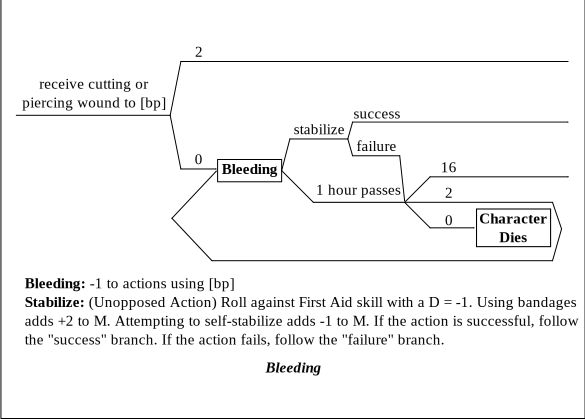
\includegraphics{svg/bleeding.eps} \end{center}


\subsection{Items and Inventory} \label{sec:items}
A character's \emdex{inventory} is the list of items carried on their person,
along with the ways in which those items are carried.
Ultimately, it is a hierarchical listing of containers and items.
Yes... it is another tree!
The root nodes of the inventory tree are the character's ``natural'' containers (hands, back, etc.),
\index{inventory!root nodes}
the intermediate nodes are containers (which are themselves items),
and the leaf nodes are arbitrary items.
The GM should specify inventory tree root nodes for each creature.

\emph{Items}\index{item} are material entities in the world, 
specifically ones that a character would carry.
Like characters, they are represented by their \emph{traits}.
\index{item traits}

\textbf{Item Traits}
\vspace{-1em}
\begin{itemize}
\item \emph{Characteristics} are item descriptors (e.g. name, textual description, material, shape)
\item \emph{Attributes} are numerical traits (e.g. weight, size, condition).
\item \emph{Conditions} are binary statuses (e.g. broken handle).
\end{itemize}

Not all items need to be represented at the same level of detail.
For many items, an item name may suffice.

The inventory tree should be subject to some constraints
\index{inventory!constraints}
(e.g. due to container volumes, character strength, fatigue, etc.).
The GM should decide how to manage these constraints
(e.g. containers have a volume attribute, characters have a carrying capacity based on some physical ability, etc.).

The GM should decide how inventories start out for each character.

\section{Actions}\label{sec:actions}
When a character attempts a task that has a possibility of failure, the outcome is governed partly by a dice roll.
The dice roll represents the dependence of the outcome on factors that are not modeled in the game or that are altogether unpredictable.
We will call these \emdex{purely variable} factors.
The basic idea is that the attempt is a success if
$$ R + M > D, $$
where $R$ is the result of a \emph{roll}, $M$ is some sort of \emdex{modifier} based on an ability level,
and $D$ is the \emdex{difficulty level} of the task.
The \emdex{relative performance} $\rho$ of the character during the action is the difference
$$ \rho=R+M-D. $$
The specifics depend on the type of action: opposed or unopposed.

When different orders\index{order} of level are used for $M$ and $D$,
no roll is necessary to resolve the action.
It is automatic success if $M$ is of a higher order than $D$, and an automatic failure
if $M$ is of a lower order than $D$.
The relative performance in those cases can be taken to be $+\infty$ and $-\infty$ respectively.


Let us use the term \emdex{aiding factors} to refer to
the primary factors leading to the possibilities of success or failure for an action,
but only those factors that are \emph{due to the character attempting the action}.
For those factors that \emph{are independent of the character attempting the action} let us use the term \emdex{difficulty factors}.
The difficulty factors for a character attempting to climb a cliff are things
like the steepness of the cliff and the availability of footholds.
The climbing skill of the character and the fact that they have a grappling hook would be aiding factors.
The difficulty factors for a character attempting to punch someone in a brawl might include the defensive abilities of the opponent,
while the punching abilities of the character would be aiding factors.
A rule of thumb is that if a factor can be removed from the picture by changing who is attempting an action,
then it is an aiding factor. Otherwise, it is a difficulty factor.

\subsection{Unopposed Actions}\label{sec:unopposed}
If the difficulty factors for an action cannot be attributed to some other character's abilities,
then the action is \emph{unopposed}.\index{action!unopposed}
In this case:
\vspace{-1em}
\begin{itemize}
\item $R$ is the result of rolling $4$dF.
\item $M$ is determined based on the aiding factors for the action; it is usually the level of an ability.
\item $D$ is determined based on the difficulty factors for the action.
\end{itemize}
Some judgement is needed for the determination of $M$ and $D$. For $M$\index{modifier},
find a skill to serve as the primary aiding factor for the character's action,
and set $M$ to be the level of that skill.
If no suitable skill is available, you may use a suitable attribute...
with a possible \emdex{attribute penalty}.\footnote{
The attribute penalty does not apply to attributes that became skills for NPCs with trimmed trees.}
If the attribute description really nails the aiding factors, then no penalty is needed.
But if the attribute is being used as a stand-in for a more specific ability that happens not to be in the ability tree,
then set $M$ to be two less than the level of that attribute.
In uncertain and in-between situations, set $M$ to be one less than the level of the attribute.
Finally, the GM should use their judgement to modify $M$ a bit further based on any other aiding factors.
Making reasonable decisions about the numbers here requires a proper understanding of section \ref{sec:quant}.
This is even more crucial for $D$, which is left completely up to the judgement of the GM.

Summarizing, an unopposed action is successful if
\begin{align*}
4\text{dF}
+([\text{relevant ability level}]
-[\text{attribute penalty}]
+[\text{other aiding factors}])
> D.
\end{align*}
The value of $R$ can feed directly into the narrative,
for it represents the purely variable aspect of a character's performance of a task,
independent of aiding factors and difficulty factors.
The same goes for the relative performance $\rho=R+M-D$, which represents actual performance given all the information.
It can be fun to asssign extreme narrative interpretations to extreme values of $R$ and $\rho$,
or even throw in some actual consequences.


\subsection{Opposed Actions}\label{sec:opposed}
If the difficulty factors for an action are due to some other character's abilities,
then the action is \emph{opposed}\index{action!opposed}, and we refer to this other character 
as the \emdex{opposing character}\index{opposing character}.
In this case:
\vspace{-1em}
\begin{itemize}
\item $R$ is $2$dF.
\item $M$ is determined based on the aiding factors for the action; it is usually an ability level of the acting character.
\item $D$ is $R' + M'$, where
\begin{itemize}
\item $R'$ is $2$dF.
\item $M'$ is determined based on the difficulty factors for the action; it is usually an ability level of the opposing character.
\end{itemize}
\end{itemize}
Here $M$ and $M'$ are determined just like $M$ for unopposed actions\index{modifier}.
Summarizing, an opposed action is successful if
\begin{align*}
&2\text{dF}
+([\text{relevant ability level}]
-[\text{attribute penalty}]
+[\text{other aiding factors}])\\
>\ & 
2\text{dF}
+([\text{relevant opposing ability level}]
-[\text{attribute penalty}]
+[\text{other difficulty factors}]).
\end{align*}
For the purpose of feeding the outcomes of rolls into the narrative,
$R$ represents the purely variable aspect of the acting character's performance,
while $R'$ represents the purely variable aspect of the opposing character's performance.
It makes sense to have the respective acting and opposing players roll the dice for these (or for the GM to roll the dice for an opposing character that is not a player).
As with unopposed actions, extreme values of $R$, $R'$,
and the relative performance $\rho=(R+M)-(R'+M')$
can be given special narrative interpretations or consequences.


\subsection{Time and Space}

For some actions it may be desirable to focus on the time they take to carry out
or on the location of the character doing them.
To handle this we can divide up time into discrete \emph{rounds} and divide up space into a \emph{grid}.
The canonical example is combat, which is coming in section \ref{sec:qombat}.

\paragraph{Rounds}
Some actions \emph{trigger rounds}\index{round},
meaning that play for everyone involved starts to proceed in a simultaneous-turn-based style,
round by round.
Each round represents the passage of a certain amount of time.
After creating an ability tree, the GM should consider various actions
that could use the various skills and decide on the following:
\vspace{-1em}
\begin{enumerate}
\item\label{itm:rounds:trigger}
Will this action ever trigger rounds? Under what circumstances?
\item\label{itm:rounds:length}
How long does it take to complete this action? (How long should a round be?)
\item\label{itm:rounds:end}
When does this action allow play to return to normal?
\end{enumerate}
Often multiple actions will trigger rounds 
(e.g. the many different combat actions coming from a combat-heavy ability tree).
It is then the greatest common divisor of the answers to \ref{itm:rounds:length} that determines round duration,
and play returns to normal when the conditions of \ref{itm:rounds:end} are met for \emph{all} the round-triggering actions involved.
When some actions take longer than the round duration, players are responsible for keeping track of their partial progress towards
the completion of an action.
For even more detail, the GM could construct some multi-component actions and answer the following in place of \ref{itm:rounds:length}:
\vspace{-1em}
\begin{itemize}
\item What are the components of this action? (Describe them for narrative purposes.)
\item How long does each component take? Does the duration depend on success or failure?
\item Can any given component be interrupted? What would interrupt it, and what would be the result?
\end{itemize}
An example could be nocking an arrow, aiming, drawing a bow, and releasing.
Such a ``high resolution'' is probably too much most of the time, so multi-component actions could be ``blurred'' into a single
action (with duration the sum of the durations of the components) until other actions get involved and shorten the round durations.

\paragraph{Location}
Some actions \emph{trigger location tracking}\index{location tracking},
meaning that the GM and the players begin to keep track of the locations of characters relative to various objects.
This can be done on a grid\index{grid} extending through the primary plane of activity
(usually a top-view grid, possibly with elevation information),
or along a more complex curve or surface if needed.
The grid/curve/surface may be represented on a board or piece of paper, but it could also just be briefly represented mentally.
For example, a detailed battle could be drawn out on a top-view grid,
but if characters are simply chasing a chicken then it suffices to mentally keep track
of their positions along the trajectory of the chicken.
After creating an ability tree, the GM should consider various actions
that could use the various skills and decide on the following:
\vspace{-1em}
\begin{enumerate}
\item\label{itm:grid:trigger}
Does part of this action ever need to be resolved with location tracking? Under what circumstances?
\item\label{itm:grid:length}
What are the spatial parameters/constraints of the action? (e.g. its range of influence, distance or placement of targets, etc.)
\end{enumerate}
The type of location tracking and its scale may be decided by the GM when it is triggered.



\paragraph{Motion}
When time is being measured in rounds \emph{and} locations are being tracked,
the relation between them brings character movement into the quantified realm.
The GM should consider the following for each creature of their world:
\vspace{-1em}
\begin{enumerate}
\item What are the main modes of locomotion\index{locomotion} for this creature? (e.g. walking, running, sprinting)
\item What is the speed of a typical one of these creatures when engaging in each mode of locomotion?
We call these \emph{base speeds}\index{base speed}.
\item Is there an ability whose training would improve this creature's speed?
\end{enumerate}
If there is such an ability, then actual speeds\index{speed}
for particular characters can be taken to be
$$ [\text{base speed}]\times (1.2)^{[\text{ability level}]} $$
for each mode of locomotion.
Otherwise, just use the base speeds directly.
Other mechanics a GM might include to constrain things are a fatigue/energy bar
or penalties due to health conditions or inventory weights.


\section{Modules}

Modules\index{module} are optional collections of rules that add certain details to the \peupfudge{} experience.
When creating their campaign, the GM should choose the modules they'd like to use
(or invent them if needed).

\subsection{Combat}\label{sec:qombat}

\def\NDF{\Delta}
\def\ODF{d}
\def\ODFA{d_A}
\def\ODFM{d_M}
\def\DDF{\ODF'}
\def\DDFA{\ODFA'}
\def\DDFM{\ODFM'}


Without saying any more, mechanics are already in place for combat:
it is a series of opposed actions that usually trigger rounds.
But a combat-heavy campaign could surely benefit from more detailed mechanics.
The combat module we build up in this section provides
a more detailed framework for resolving an attack.

\subsubsection{Attack Terminology}
For clarity of language we will call the acting character the \emdex{attacker}
and the opposing character the \emdex{defender}.
%There are four types of factors that determine the outcome of an attack.
We also call the aiding factors \emdex{hitting factors} and we call the difficulty factors
\emdex{preventive factors}.
These determine the \emph{success}\index{attack success} of an attack. There are two other types of factors that
contribute only to its \emph{effectiveness}\index{attack effectiveness} in the event of success:
\emdex{impact factors} and \emdex{protective factors}.
Laying out the four types of factors that contribute to attack resolution, we have:
\vspace{-1em}\begin{itemize}
\item \emph{Hitting factors} are involved in determining whether an attack hits the defender,
and they are those factors that depend on who is attacking.
\item \emph{Preventive factors} are also involved in determining whether an attack hits the defender,
but independently of who is attacking. 
\item \emph{Impact factors} contribute only to the damage a successful attack can inflict on its target
(not to its chances of success in the first place),
and they are those factors that depend on who is attacking.
\item \emph{Protective factors} also contribute only to damage inflicted,
but independently of who is attacking.
\end{itemize}
\begin{center}\begin{tabular}{l|ll}
              & offensive & defensive  \\
\cline{1-3}
success       & hitting   & prevention \\
effectiveness & impact    & protection 
\end{tabular}\end{center}
%Imagine, for example, an attacker lunging with a sword at an armored defender:
Consider the example of an attacker lunging with a sword at an armored defender.
%In the example, one hitting factor might be the sword skill of the attacker.
The attacker's sword skill is a hitting factor,
%In the example, one preventive factor might be the dodging skill of the defender.
and defender's dodging skill is a preventive factor.
Now consider what happens if the lunge strikes its target.
%In the example, one impact factor might be the strength skill of the attacker.
The attacker's strength is an impact factor,
%In the example, one protective factor might be the type of armor the defender is wearing.
and the defender's armor is a protective factor.
%It should be noted that the line between offensive and defensive factors is not always clear. Some factors will be dependent on both the attacker and the defender. For example, if an attacker sneaks up on an unsuspecting defender, the chance of a successful attack will increase; but would that be because the attacker is sneaking or because the defender is caught by surprise? Because the factors are summed together, in such a case, the element of surprise can be considered as either a hitting factor or a preventive factor; just make sure not to count its effect twice.


\subsubsection{Abilities for Combat}
There are two ways in which abilities play a role in attack resolution:
to determine whether an attack is successful
and to determine how effective it is.
When designing an ability tree, the GM
should ensure that it has an adequate set of abilities
to accommodate combat.
First, make a list of attacks that you think players could attempt in this world.
Go through all the skills and consider, for each skill, how a player might try and use the skill
in the context of an attack. Add these attacks to the list.
Now go through all the attacks in your list and ask the following of each attack:
\vspace{-1em}\begin{itemize}
\item Is it clear which ability would be relevant to determining whether the attack is successful?
\item Is it clear which ability or abilities would be relevant to determining the effectiveness of the attack?
\end{itemize}
Add or rearrange abilities until these questions can be answered satisfactorily.

\subsubsection{Resolving an Attack}
During a combat round, a player who is able to attack\index{attack} another player (e.g. is within range) may attempt to do so.
Here is the attack resolution process:
\vspace{-1em}\begin{enumerate}
\item
An attack is an opposed action, resolved according to relative performance:
$$ \rho = (R + M) - (R' + M'). $$
A negative value is a \emdex{miss}, a positive value is a \emdex{hit}, and a value of zero is a \emdex{graze}.
The modifiers $M$ and $M'$ are comprised of several bits that are explained in section \ref{sec:sitmod}.
\item
In the case of a miss, attack resolution is complete.
Otherwise determine the target of the attack, by rolling if needed (see section \ref{sec:bodyparts}).
\item
%In the case of a hit or a graze, further rolling is done to determine the severity of the outcome,
Quantify the severity of the outcome as \emdex{damage}.
Computing damage requires settling on a \emph{damage factor} $\NDF$ for the attack, explained in section \ref{sec:ndf}.
A hit results in a damage of
$$ \rho + \NDF $$
while a graze results in a damage of
$$ \frac{1}{2} \NDF, $$
rounding down.
\item
Damage then determines the type of wound\index{wound} inflicted on the target, according to section \ref{sec:wounds}.
\item
Consider what health conditions have developed, and the penalties that can influence later attacks.
\end{enumerate}

When $M$ is of a lower or greater order\index{order} than $M'$, hit damage is taken to be $0$ or $\infty$ respectively.
In this case there would be no need to consider $\NDF$.


\subsubsection{The Modifiers $M$ and $M'$}\label{sec:sitmod}


\paragraph{Situation}
Many factors having to do with the particular situation\index{situation}
surrounding an attack can be tossed into the determination of $M$ and $M'$.
Focus on
aspects of the situation that affect the attack's probability of success,
and less on the expected effectiveness of the strike in the
event of success (the latter is accounted for in impact and protection).
Here are some suggestions for situations to consider:
\vspace{-1em}\begin{itemize}
\item Weapon lengths/types. A knife-wielder is at a disadvantage defending themselves against an attacking sword-wielder.
\item Weapon condition. A properly balanced sword or a properly sighted rifle improve chances of a successful strike.
\item Cover. Someone behind cover has a defensive advantage in the face of enemy gunfire.
\item Range. A distant target is more difficult to hit with a ranged weapon.
\item Multiple attackers. Someone facing multiple attacks at the same time has more trouble defending themselves.
\item Injuries. An injured person can have some trouble defending as well as attacking.
\item Surprise. Being caught off-guard lowers one's chances of a successful defense.
\item Scale. A huge character can be much easier to hit, a small character much harder.
\item Positioning. Melee combat can be affected by things like bad footing,
lower elevation, light in eyes, kneeling, etc. %I finally found this on fudge manual p35
\end{itemize}




\paragraph{Stance}
At the beginning of each round of combat,
characters have an opportunity to choose a \emdex{stance}:
defensive ($-1$), balanced ($0$), or aggressive ($1$).
This number is added to a character's $M$ for their attack and subtracted from their
$M'$ each time they are attacked during the round.
A balanced stance is assumed if no stance is explicitly chosen.


\paragraph{Targeting}
A player may call, before their attack is resolved, that they intend to target a certain body part.
This introduces a \emdex{targeting penalty} that decreases $M$, based on the difficulty of hitting that body part.
The GM judges what the targeting penalty should be;
to give a frame of reference it could be $1$ for a torso and $4$ for an eye.
If the player does not miss, then one records in addition to the usual wounds the specific body part that received the wound.


\subsubsection{Body Parts}\label{sec:bodyparts}

%gm should create body diagram for each creature, with sizes of body parts included.
For each creature of their world, the GM should create a body diagram\index{body diagram}
that indicates relative sizes of body
parts that can serve as targets and be injured in combat.
Here is an example for humans:
%example of it for human
\begin{center} 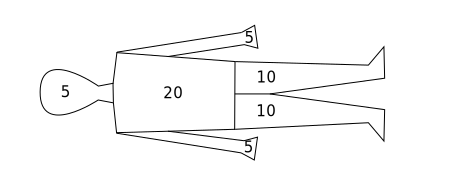
\includegraphics{svg/bp1.eps} \end{center}

%roll to determine target if no targetting was called
If no target was called by the attacking player before their attack was resolved, then a target
for the attack is chosen at random. The choice is weighted by body part size,
and it can be determined by a roll.
Mangled body parts (see section \ref{sec:wounds}) should not be included in target choice--
simply re-roll if they come up as a target.
%convert sizes to die rolls for the purpose of randomly choosing a body part, with weighting by size
Actually, the GM should convert relative body part sizes into dice roll ranges
and present the body diagram with this included.
Here is our example with d$20$ ranges put in:

%example of die roll labels for human
\begin{center} 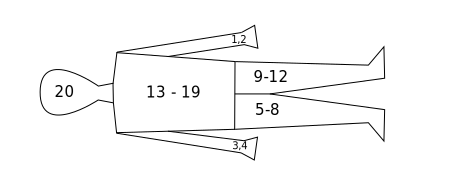
\includegraphics{svg/bp2.eps} \end{center}

\subsubsection{Impact and Protection}\label{sec:ndf}
The damage dealt by a successful attack depends on the \emdex{damage factor} $\NDF$,
the difference between \emdex{impact} and \emdex{protection}:
$$ \NDF = \text{[impact]} - \text{[protection]}. $$
%Impact is given by the impact factors, which are the factors that determine the capability of the attack to deal damage.
%The offensive damage factor $\ODF$ is defined to be the sum of the factors that determine the capability of the attack to deal damage,
%and the defensive damage factor $\DDF$ is defined to be the sum of the factors that determine the defender's capacity to absorb damage.level $\ODFA$ of a relevant ability
%plus a damage modifier $\ODFM$, and similarly for $\DDF$.
%The ability that goes into $\ODFA$ should be one that plays a role in determining how
%powerful the attack is (e.g. strength for an axe swing), and the ability that goes into $\DDFA$
%should be one that plays a role in determining a character's capacity to absorb damage (e.g. constitution). 
%If no relevant ability can be identified for $\ODFA$ or $\DDFA$, set it to $0$. 
%The damage modifer consists of other factors that affect the ability of the attack to do damage.
%For example $\ODFM$ could involve the weapon being used, and $\DDFM$ could involve the defender's armor.
%Putting it together,
%$$ \NDF = (\ODFA + \ODFM) - (\DDFA + \DDFM). $$
Impact is a sum of effects coming from the impact factors involved in the attack,
and protection is a sum of effects coming from protection factors.
Let us go through some of the factors that should be included.

\paragraph{Abilities}
The level of a relevant ability can be included directly in impact.
Or, if it only partly applies, a lesser portion of the ability level may be used.
For example a stronger character deals a deadlier blow with a melee weapon, so a strength ability could be used.
Don't stack the effects of multiple abilities; instead, use the nearest common ancestor attribute when multiple abilities apply.
A relevant ability may also be included, separately, in protection.
For example a tougher character can take a harder hit without receiving as much of an injury.

\paragraph{Size}
The same blow imparts greater destruction to smaller targets. 
This is why the \emdex{size} of a target is important to protection.
When creating their world, the GM should choose a \emdex{baseline target}
size with respect to which all target sizes are compared.
The choice of baseline target calibrates the entire damage system to respond appropriately to target sizes.
A good baseline target is one that, with all other things being equal, would be injured a bit from a good punch.
More precisely, it is a target that recieves a wound of degree $1$ (see section \ref{sec:wounds}) about $38\%$
of the time, and a wound of degree $0$ the rest of the time, from a successful unarmed attack by an equally matched standard being.
%use the protection table to determine suitable contribution to protection due to size of body part
Use the following table to choose a suitable contribution to protection due to the size of a body part:
\begin{center}
\input{size_protection_table.tex}
\end{center}
Sizes are measured in in units of the baseline target size,
and the value in the right hand column is included in the calculation of total protection.
%we recommend just putting this number on the body charts directly
Actually, the GM can include these protection modifiers on the body diagram\index{body diagram}
directly for players' convenience.
%example for human, with torso as baseline target
Here is our human example from above, with protection modifiers included,
using a human torso as the baseline target:

\begin{center} 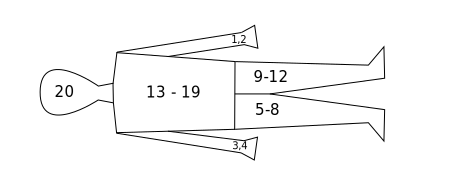
\includegraphics{svg/bp3.eps} \end{center}

\paragraph{Other Things}
We list below suggestions for some other factors that can be included.
An understanding of section \ref{sec:wounds} is required for the GM to properly
judge the contribution of these factors to impact and protection.
\vspace{-1em}\begin{itemize}
\item Weapon quality. A sharp sword has a greater impact than a dull or worn sword.
\item Weapon type. A knife has greater impact than a fist.
As a baseline for this modifier, a contribution of $0$ to impact
can be attributed to an unarmed attack by the standard being.
\item Armor, natural or otherwise. A creature with a tough exterior or armored clothing has greater protection.
\end{itemize}


\subsubsection{Wounds}\label{sec:wounds}

%intro
%hp of body parts
Wounds on body parts are tracked in terms of \emdex{hit points} (hp).
Each body part of each character has a number of hit points ranging from
$0$ to $4$.
%wound of 'degree' x
When damage dealt to a target body part results in a decrease of its hp by an amount $n$, 
a \emph{wound of degree}\index{wound degree}
$n$ is said to have been inflicted upon the target.
%damage dealt is according to following table. record new hp. on body diagram, why not.
Use the following table to determine the degree of wound inflicted on a defender's body part
due to a given damage:
\begin{center}
\input{damage_table.tex}
\end{center}
Players should keep track of the hp values of body parts of the characters under their control;
the body diagram is a useful place to record this information.

%pay attention to health peups that could have been triggered
Some health conditions may have developed following a wound;
remember to consider how resulting penalties can influence later attacks.

%death
The defender dies if a \emdex{vital body part} is at an hp of $0$.
The GM should decide, for each creature of their world, which body parts are vital.

%narrative interpretation of wounds
The hp values for a body part have the following descriptions that can feed into the narrative:
\begin{center}
{\setlength{\extrarowheight}{1pt}
\begin{tabular}{l|l}
hp & adjective \\
\cline{1-2}
4  & fine \\
3  & scratched \\
2  & hurt \\
1  & incapacitated \\
0  & mangled
\end{tabular}}
\end{center}

\paragraph{Healing} Wounds are treated like any other health condition, so healing\index{healing} is governed by a flowchart.
After deciding on the creatures that inhabit their world, the GM should devise for each one a healing flowchart.
Here is a somewhat generic healing flowchart geared towards organic creatures:
\begin{center} 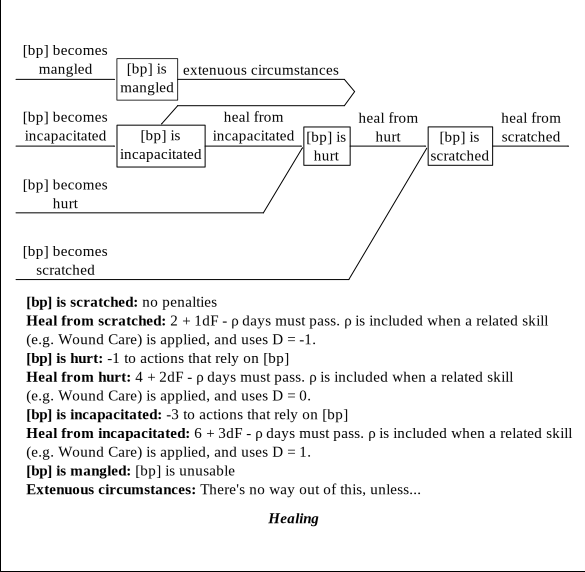
\includegraphics{svg/healing.eps} \end{center}




\section{Appendix}

\subsection{Campaign Setup Checklist}

There are many rules throughout this manual that depend
on a GM decision that had to be made during the creation of their campaign.
As a convenient checklist, we restate those decision points here.

\begin{enumerate}
\item What is the standard being?
\item What character characteristics are relevant to the campaign?
\item Are there any predefined properties? Are characters limited to these?
\item What are the bars? For each bar:
\begin{enumerate}
  \item What values/states can the bar be in, and what do the different states mean?
  \item What causes the bar to change state? Also, how does it start out?
  \item What are the effects of the bar's being in the various states?
\end{enumerate}
\item For each creature type, what health conditions exist for it? Make flowcharts.
\item Set up the inventory system:
\begin{enumerate}
  \item For each creature type, what are the root nodes of its inventory tree?
  \item How are inventory trees constrained?
  \item Are there any predefined items?
  \item How will player character inventories start out?
\end{enumerate}
\item Set up the ability tree:
\begin{enumerate}
  \item Make an ability tree.
        This includes naming abilities,
        choosing their starting levels,
        connecting abilities by arrows to form a tree,
        and labeling the arrows with weights.
  \item For each ability, consider it in the context of the creatures of the world. Does it need any special order labels?
  \item For each ability, consider various actions that could use it.
  \begin{enumerate}
    \item Does the action ever trigger rounds? If so:
    \begin{enumerate}
      \item Under what circumstances?
      \item Is it a multi-component action? If so, can it be interrupted?
      \item How long does it take to complete the action? If it is a multi-component action, what is the duration of each component?
      \item When does play return to normal?
    \end{enumerate}
    \item Does the action ever need to be resolved with location tracking? If so:
    \begin{enumerate}
      \item What are the spatial parameters/constraints for the action?
    \end{enumerate}
  \end{enumerate}
  \item Are there any abilities that should be powers?
  \begin{enumerate}
    \item For each power, what circumstances cause it to become enabled or disabled?
  \end{enumerate}
\end{enumerate}
\item Set up character creation:
\begin{enumerate}
  \item Are there any predefined classes (pretrained trees)? Do players need to pick from these classes?
  \item How much xp do players start with for character creation?
\end{enumerate}
\item For each creature type, what are its modes of locomotion?
\begin{enumerate}
  \item What is the base speed of a typical one of these creatures when engaging in each mode of locomotion?
  \item Is there an ability whose training would improve this creature's speed?
  \item Are speeds constrained in any other way (e.g. by some bars)?
\end{enumerate}
\item Design a blank character sheet and make any reference sheets players could use.
\begin{enumerate}
  \item Put dice roll thresholds on ability tree arrows in place of weight labels.
\end{enumerate}
\item What modules will you use?
\begin{enumerate}
  \item If you include the Combat module:
  \begin{enumerate}
    \item What is the baseline target size?
    \item For each skill, how might a player use this skill in the context of an attack? For each attack:
    \begin{enumerate}
      \item Is it clear which ability is most relevant to determining whether the attack succeeds?
      \item Is it clear which ability is most relevant to the attack's effectiveness?
    \end{enumerate}
    \item For each creature type:
    \begin{enumerate}
      \item Make a body diagram that indicates the possible targets of attacks. Quantify relative sizes of body parts.
      \item Add dice rolls for random target selection to the body diagram.
      \item Add protection modifiers to the body diagram.
      \item Which body parts are vital?
      \item Make or choose a healing flowchart for wounds.
    \end{enumerate}
  \end{enumerate}
\end{enumerate}
\end{enumerate}


\printindex

\end{document}
